\documentclass{article}
\usepackage{amsmath}
\usepackage{graphicx}
\usepackage{listings}
\usepackage{xcolor}
\usepackage{siunitx}
\usepackage[T1]{fontenc}
\usepackage[italian]{babel}
\usepackage[utf8]{inputenc}
\usepackage{tikz} % Pacchetto per disegnare grafica
\usetikzlibrary{patterns} % Libreria opzionale per motivi e modelli
\title{Introduzione alla Distribuzione Gaussiana}
\author{Nome dell'Insegnante}
\date{}

% Definizione dello stile per il codice Python
\lstdefinestyle{pythonstyle}{
    language=Python,
    basicstyle=\ttfamily\small,
    keywordstyle=\color{blue},
    commentstyle=\color{gray}, % Cambiato il colore dei commenti
    stringstyle=\color{red},
    numbers=none, % Rimosso i numeri di riga
    backgroundcolor=\color{lightgray},
    frame=single,
    tabsize=4,
    breaklines=true,
    showstringspaces=false,
    captionpos=b
}

\begin{document}

\maketitle

\section{Introduzione}
La distribuzione gaussiana, nota anche come distribuzione normale, è una delle più importanti distribuzioni di probabilità in statistica e nelle scienze naturali. Molte grandezze fisiche e biologiche, quando vengono misurate, tendono a seguire una distribuzione normale, soprattutto quando sono influenzate da un gran numero di piccoli effetti casuali indipendenti. Un esempio classico è l'altezza delle persone in una popolazione.

\section{Distribuzione di Probabilità}
In questa e nelle prossime sezioni, parleremo di probabilità. Quando misuriamo una grandezza casuale, vediamo che alcuni valori si ripetono più frequentemente di altri, ossia abbiamo una \textit{distribuzione} di valori. La statistica ci permette di estrarre da questa distribuzione, informazioni sulla grandezza. Si suppone che ogni grandezza abbia un valore ''vero`` e che solo effetti casuali discostino il risultato da quest'ultimo. La distribuzione dei valori viene misurata non tanto dalla semidispersione massima (una stima troppo grande) ma dalla deviazione standard (il nostro famoso errore assoluto nel caso di misure ripetute). Ripetendo le misure molte volte, costruendo un  particolare grafico chiamato \textbf{istogramma delle frequenze}, otteniamo che questo istogramma diventa sempre  più liscio e  si avvicina ad una curva a forma di campana. In fisica, questa curva si presenta quando ripetiamo molte volte una misura casuale. In quel caso, la grandezza non ha sempre lo stesso valore ma ha, appunto, una \textit{distribuzione}. Se facciamo oscillare un pendolo, e misuriamo la durata $t$ di 20 oscillazioni con un cronometro manuale, non otterremo quasi mai due volte lo stesso valore (a causa di errori umani) ma una serie di valori. La statistica ci consente di prevedere quali saranno i valori più probabili e come questi si distribuiscono, (quanti ad esempio sono molto più grandi o più piccoli della media). Le prossime sezioni ci insegneranno come trarre informazioni utili dalla distribuzione di queste misure. Impareremo che il risultato di una misura è dato dalla media e dall'errore della media, come segue:
\[
x=\left(\overline{x} \pm \sigma_{\overline{x}}\right) \, \text{u.m.}
\]
essendo $\overline{x}$ la media dei valori e $\sigma_{\overline{x}}$ la cosiddetta deviazione standard della media.

\subsection{La Curva di Gauss}

La distribuzione gaussiana è caratterizzata dalla seguente funzione densità di probabilità (pdf):

\begin{equation}
f(x|\mu,\sigma) = \frac{1}{\sigma \sqrt{2\pi}} e^{-\frac{(x-\mu)^2}{2\sigma^2}}
\end{equation}

dove:
\begin{itemize}
    \item $\mu$ è la media della distribuzione, che indica il valore centrale attorno al quale i dati sono distribuiti.
    \item $\sigma$ è la deviazione standard, che misura la dispersione dei dati rispetto alla media.
\end{itemize}

La curva di Gauss ha una forma a campana, simmetrica rispetto alla media $\mu$. La maggior parte dei dati (circa il 68\%) si trova entro un intervallo di una deviazione standard dalla media ($\mu \pm \sigma$), mentre il 95\% dei dati si trova entro due deviazioni standard ($\mu \pm 2\sigma$). Questo comportamento rende la distribuzione gaussiana particolarmente utile per descrivere fenomeni naturali dove le variazioni sono dovute a molti fattori piccoli e indipendenti. In figura \ref{fig:curva_gaussiana} vediamo il tipico aspetto di una gaussiana.

\begin{figure}[h!]
    \centering
     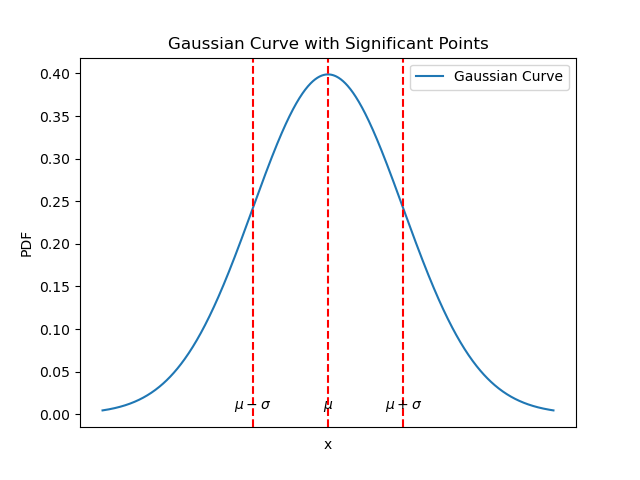
\includegraphics[scale=0.7]{curva_gaussiana.png} 
    \caption{Curva Gaussiana con Evidenziati \(\overline{x}\), \(\overline{x} - \sigma\), e \(\overline{x} + \sigma\)}
    \label{fig:curva_gaussiana}
\end{figure}


\section{Istogrammi a Bins}
Un istogramma è una rappresentazione grafica della distribuzione di un insieme di dati. Esso suddivide l'intervallo dei dati in una serie di intervalli chiamati bins (o classi) e conta il numero di dati che rientrano in ciascun bin. L'altezza di un rettangolo è pari alla frequenza, ossia è pari al rapporto tra le misure  comprese tra i due estremi della base del rettangolo  e il totale delle misure.  In figura \ref{fig:istogrammagenerico} vediamo un tipico istogramma.

\begin{figure}[h!]
    \centering
    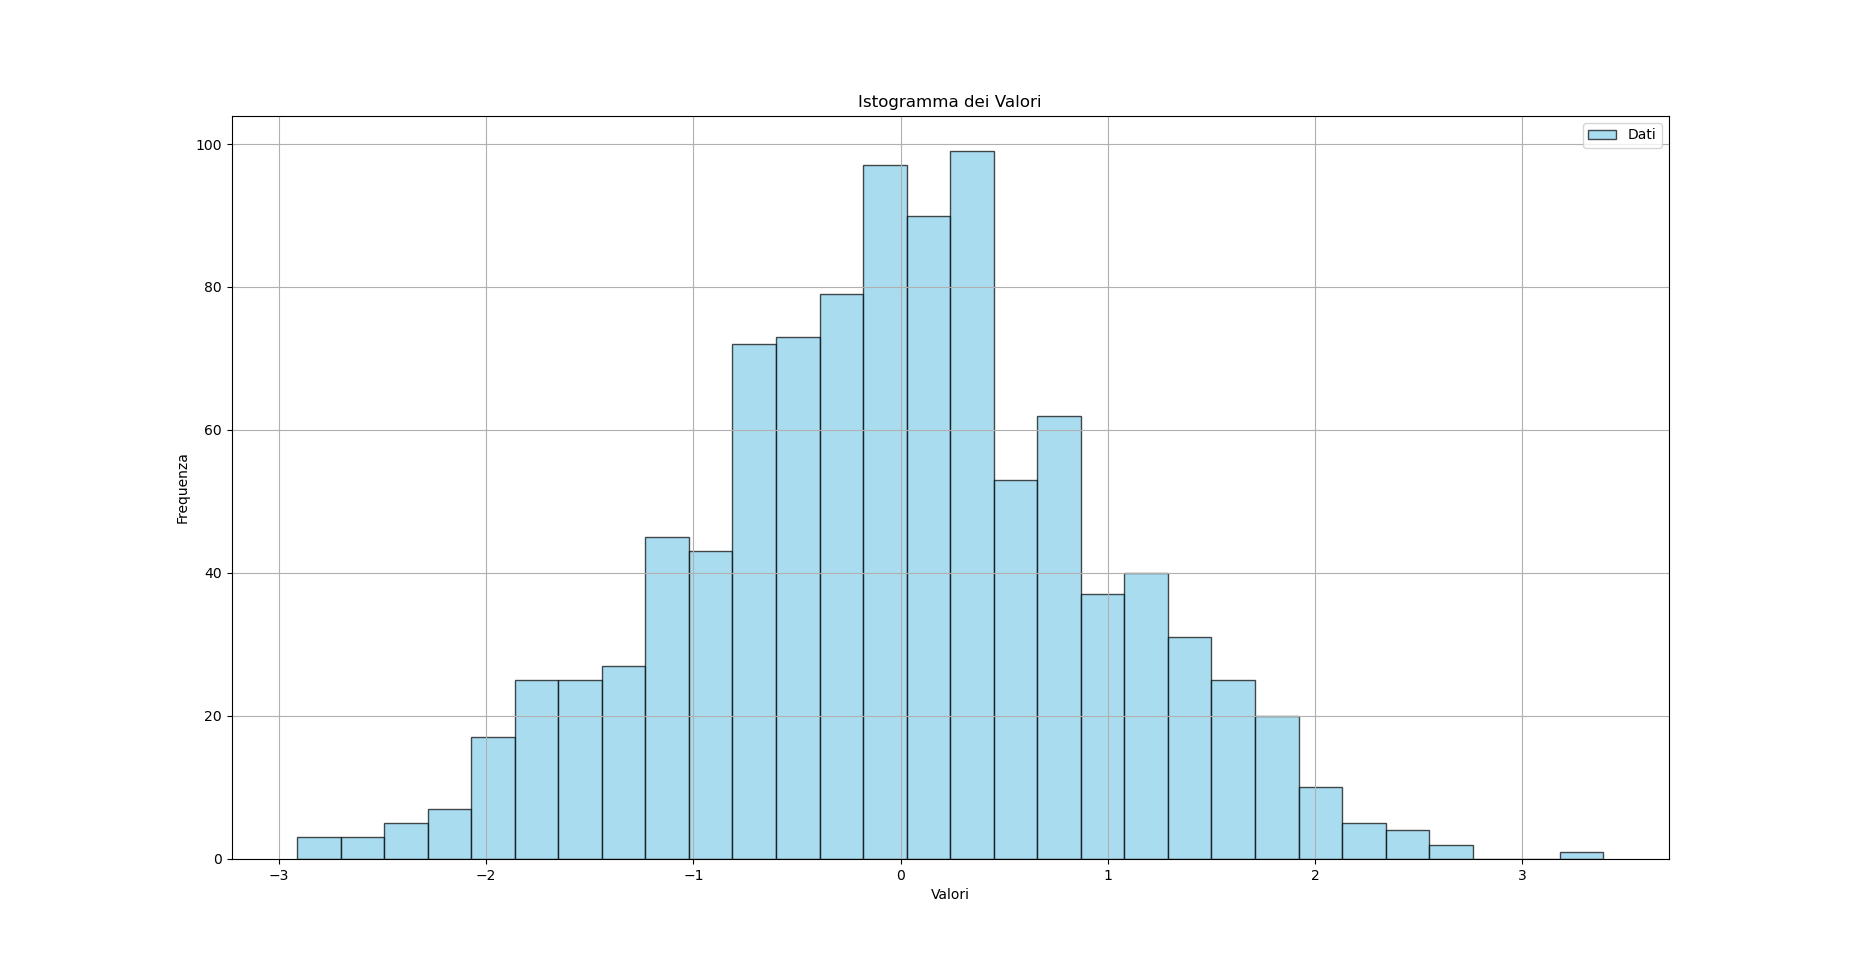
\includegraphics[width=\linewidth]{istogrammagenerico.png}
    \caption{Istogramma dei Valori}
    \label{fig:istogrammagenerico}
\end{figure}


 
L'ampiezza dei bins può influenzare significativamente l'aspetto dell'istogramma. Bins più stretti possono mostrare più dettagli, ma possono anche evidenziare il rumore nei dati, mentre bins più larghi forniscono una visione più smussata della distribuzione. La scelta del numero di suddivisioni dipende dal numero di dati: se si hanno molti dati si possono prendere più bins. Si consiglia di fare dei tentativi. Se l'istogramma rappresenta una distribuzione gaussiana  (detta anche ''normale``) il suo aspetto deve ricordare quello di una campana. Ne parleremo nei prossimi paragrafi in cui useremo il linguaggio Python per disegnare un'istogramma. Questo linguaggio offre maggiori personalizzazioni dei semplici grafici realizzati da excel.Il grafico in figura è stato realizzato col codice python:

\begin{lstlisting}[style=pythonstyle, caption={Script Python per disegnare un'istogramma}]
import matplotlib.pyplot as plt
import numpy as np

# Dati di esempio
data = np.random.randn(1000)

# Creazione della figura e dell'asse
fig, ax = plt.subplots()

# Creazione dell'istogramma
n, bins, patches = ax.hist(data, bins=30, color='skyblue', edgecolor='black', alpha=0.7)

# Aggiunta di etichette agli assi
ax.set_xlabel('Valori')
ax.set_ylabel('Frequenza')

# Aggiunta di un titolo
ax.set_title('Istogramma dei Valori')

# Aggiunta di una legenda
ax.legend(['Dati'])

# Aggiunta di una griglia
ax.grid(True)

# Mostra il grafico
plt.show()



\end{lstlisting}



\section{Approssimazione della Gaussiana}
In un esperimento, se ripetiamo molte volte una misura e calcoliamo la media e la deviazione standard, al crescere del numero di misure, l'istogramma dei dati approssima sempre meglio la distribuzione gaussiana. Questo è dovuto al teorema centrale del limite, il quale afferma tra l'altro che le formule per media e deviazione standard della media, se applicate a campioni di dati molto grandi, ci restituiscono proprio i valori teorici di queste grandezze che restano comunque un concetto teorico. Quando una persona fà un esperimento di misura, a quella persona e quell'apparato, corrisponde una media teorica, ossia i valori delle grandezze si sparpaglieranno in un certo modo perché quella persona e quell'apparato hanno una sorta di sensibilità: se qualcun altro fà la misura, questa si \textit{sparpaglierà} diversamente. Ad esempio, se Marco lascia cadere un pallina mille volte (povero Marco... ) e misura la media e la deviazione standard dei tempi di caduta, magari otterrà una deviazione standard di 0,8 s e una media di 0,2 s. Se facciamo cadere la pallina usando una fotocellula per misurare il tempo, le misure si sparpaglieranno di meno e avremo una deviazione standard ad esempio di 0,01 s con una media di 0,16 s. Come si vede, la grandezza da misurare (il tempo di caduta) è la stessa ma uno dei sue sistemi è più preciso (quello con la fotocellula). Se andassimo a costruire gli istogrammi sperimentali, quello della misura del ragazzo, avrebbe una forma a campana più larga perché la deviazione standard misura tra l'altro quanto è largo l'istogramma. 

\section{Stima di Media e Deviazione Standard}
Data una serie di $n$ misurazioni sperimentali $\{x_1, x_2, \ldots, x_n\}$, possiamo stimare i parametri della distribuzione gaussiana, cioè la media $\mu$ e la deviazione standard $\sigma$, utilizzando le seguenti formule:

\subsection{Calcolo della Media}
La media campionaria $\hat{\mu}$ è data dalla somma di tutte le osservazioni divisa per il numero totale di osservazioni:

\begin{equation}
\hat{\mu} = \frac{1}{n} \sum_{i=1}^{n} x_i
\end{equation}

\subsection{Calcolo della Deviazione Standard}
La deviazione standard campionaria $\hat{\sigma}$ è data dalla radice quadrata della somma dei quadrati delle differenze tra ciascuna osservazione e la media campionaria, divisa per il numero di osservazioni meno uno:

\begin{equation}
\hat{\sigma} = \sqrt{\frac{1}{n-1} \sum_{i=1}^{n} (x_i - \hat{\mu})^2}
\end{equation}

\subsection{Calcolo della Deviazione Standard della Media}
La deviazione standard della media, nota anche come errore standard della media, è calcolata come:

\begin{equation}
\sigma_{\overline{x}} = \frac{\hat{\sigma}}{\sqrt{n}}
\end{equation}

Dove $\hat{\sigma}$ è la deviazione standard campionaria e $n$ è il numero di osservazioni. La deviazione standard della media rappresenta quanto la media campionaria è attesa essere distante dalla media vera della popolazione. Per una stima più precisa, questa deviazione standard della media viene approssimata a una cifra significativa.

\section{Esempio Pratico in Python}
Per illustrare questi concetti, consideriamo un esempio pratico in Python. Abbiamo misurato le altezze di 100 persone (in cm) e calcoleremo la media, la deviazione standard e la deviazione standard della media di queste misure. Successivamente, creeremo un istogramma delle altezze e lo sovrapporremo con la curva gaussiana corrispondente.

\begin{lstlisting}[language=Python, caption={Script Python per calcolare e visualizzare le altezze}]
import numpy as np
import matplotlib.pyplot as plt
from scipy.stats import norm

# Altezze di 100 persone (in cm)
heights = [170, 165, 180, 175, 160, 155, 178, 172, 168, 169, 
           174, 167, 166, 171, 173, 177, 182, 181, 176, 179, 
           164, 163, 162, 161, 159, 158, 157, 156, 154, 153, 
           152, 151, 150, 149, 148, 147, 146, 145, 144, 143,
           150, 155, 160, 165, 170, 175, 180, 185, 190, 195,
           172, 177, 182, 187, 192, 197, 162, 167, 172, 177,
           180, 175, 170, 165, 160, 155, 150, 145, 140, 135,
           142, 147, 152, 157, 162, 167, 172, 177, 182, 187,
           165, 170, 175, 180, 185, 190, 195, 200, 205, 210]

# Stima di media, deviazione standard e deviazione standard della media
mu = np.mean(heights)
sigma = np.std(heights, ddof=1)
sigma_x_mean = sigma / np.sqrt(len(heights))

# Arrotonda la deviazione standard della media e la media alle unità
sigma_x_mean_rounded = round(sigma_x_mean)
mu_rounded = round(mu)

print(f"Media delle altezze: {mu_rounded} cm")
print(f"Deviazione standard delle altezze: {sigma:.2f} cm")
print(f"Deviazione standard della media: {sigma_x_mean_rounded} cm")

# Creazione dell'istogramma
count, bins, ignored = plt.hist(heights, bins=6, density=True, alpha=0.6, color='g', edgecolor='black')

# Sovrapposizione della curva gaussiana
xmin, xmax = plt.xlim()
x = np.linspace(xmin, xmax, 100)
p = norm.pdf(x, mu, sigma)
plt.plot(x, p, 'k', linewidth=2)
title = "Istogramma delle Altezze e Curva Gaussiana"
plt.title(title)

# Visualizzazione di media e deviazione standard
plt.axvline(mu, color='r', linestyle='dashed', linewidth=1)
plt.text(mu + mu/10, max(p), f'Media: {mu_rounded} cm', color='r')
plt.axvline(mu + sigma, color='b', linestyle='dashed', linewidth=1)
plt.axvline(mu - sigma, color='b', linestyle='dashed', linewidth=1)
plt.text(mu + sigma + mu/10, max(p)/2, f'Sigma: {sigma:.2f} cm', color='b')
plt.text(mu - sigma - mu/10, max(p)/2, f'Sigma: {sigma:.2f} cm', color='b')

# Impostazione dei valori sui bins come etichette sull'asse x
bin_labels = [f"{int(bins[i])}" for i in range(len(bins))]
plt.xticks(bins, labels=bin_labels, rotation=45)

# Migliora la disposizione dei sottotitoli e delle etichette
plt.tight_layout()

plt.savefig('istogramma.png')
plt.show()

# Risultato finale, arrotondato a due cifre significative
print(f"Altezza = ({mu_rounded} ± {sigma_x_mean_rounded}) cm")
\end{lstlisting}

\subsection{Significato delle Variabili, Moduli, Funzioni e Parametri}
Spieghiamo brevemente il significato delle variabili, dei moduli usati, delle funzioni e dei parametri:

\begin{itemize}
    \item \texttt{numpy} (\texttt{np}): Una libreria per il calcolo numerico in Python. Utilizzata per calcolare la media (\texttt{np.mean}) e la deviazione standard (\texttt{np.std}) delle altezze.
    \item \texttt{matplotlib.pyplot} (\texttt{plt}): Una libreria per la creazione di grafici. Utilizzata per creare l'istogramma (\texttt{plt.hist}) e sovrapporre la curva gaussiana (\texttt{plt.plot}).
    \item \texttt{scipy.stats.norm}: Fornisce la funzione di densità di probabilità per una distribuzione normale. Utilizzata per calcolare la curva gaussiana da sovrapporre all'istogramma.
    \item \texttt{plt.hist()}: Funzione per creare un istogramma. Il parametro \texttt{bins} definisce il numero di intervalli.
    \item \texttt{plt.plot()}: Funzione per tracciare una linea su un grafico. Utilizzata per disegnare la curva gaussiana.
    \item \texttt{np.linspace()}: Funzione per generare una sequenza di numeri spaziati uniformemente. Utilizzata per generare i valori x della curva gaussiana.
\end{itemize}

Ecco l'output:
\begin{verbatim}
Media delle altezze: 167.83333333333334 cm
Deviazione standard delle altezze: 15.80 cm
Deviazione standard della media: 1.67 cm
Altezza = (168 ± 2) cm
\end{verbatim}
Nel grafico \ref{fig:istogramma} vediamo sovrapposto l'istogramma costruito e la curva che lo approssima. L'istogramma ha in ascisse (asse X) gli intervalli di altezza e in ordinate (asse Y) un valore tale che l'area del bin sia uguale alla frazione di persone che hanno un'altezza compresa tra i suoi estremi. Ad esempio, se guardiamo l'intervallo tra 160 e 172, l'altezza è 0,025 perché $\left(172-160 \right)\times 0,025 =0,3$ ossia, il 30\% delle persone aveva un'altezza compresa tra 160 e 172 centimetri. Ancora un commento su media e deviazione standard. Notare che la curva è centrata attorno alla media (il valore $\SI{167,3}{\centi\meter}$) evidenziata dalla linea rossa tratteggiata. Notare anche le due linee blu. La distanza tra la linea verde e quella blu è proprio uguale alla deviazione standard (pari a $\SI{15,80}{\centi\meter}$ e indicata sul grafico come \textit{Sigma}), infatti $\SI{167,83}{\centi\meter} + \SI{15,80}{\centi\meter} = \SI{183,63}{\centi\meter}$ che è proprio dove si trova la linea verde. Notiamo infine che il 68\% delle misure capitano tra i valori $\SI{167,83}{\centi\meter} -\SI{15,80}{\centi\meter}$ e $\SI{167,83}{\centi\meter} +\SI{15,80}{\centi\meter}$, ossia tra $\SI{152,03}{\centi\meter}$ e $\SI{183,63}{\centi\meter}$. Questo è sempre vero. Quando abbiamo una grandezza che si distribuisce come la curva a campana (la gaussiana scoperta dallo scienziato Gauss) l'area sotto la curva, quella compresa tra le due linee blu, è sempre 0,68 ossia il 68\% delle misure che la approssimano, dovrebbero capitare tra $\overline{x} -\sigma$ e $\overline{x} + \sigma$.

\begin{figure}[h!]
    \centering
    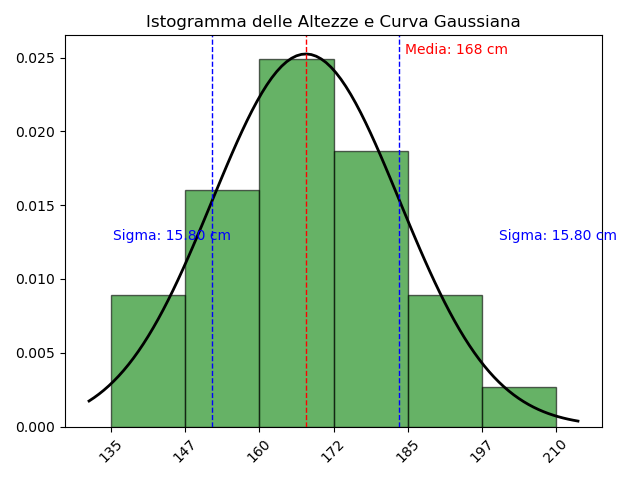
\includegraphics[width=0.8\textwidth]{istogramma.png}
    \caption{Istogramma delle Altezze con Sovrapposta la Curva Gaussiana}
    \label{fig:istogramma}
\end{figure}

\section{Conclusioni}
La distribuzione gaussiana è un modello fondamentale nella statistica e nelle scienze. La sua importanza deriva dal fatto che molti fenomeni naturali e misure sperimentali seguono una distribuzione normale. Conoscere come calcolare e interpretare la media, la deviazione standard e la deviazione standard della media ci permette di fare previsioni e inferenze più precise basate sui dati.

\end{document}
